\renewcommand\TheFile{ch04_graphics.tex}

\begin{savequote}[15cm]
  \vspace{-30mm}
  \raggedleft
  \sffamily
A picture is worth 1000 words
  \qauthor{Anonymous}
\end{savequote}
\chapter{Graphics as easy as pie}
\LaTeX, combined with pdf in \texttt{pdflatex}, supports the following
graphic file types: pdf, png, jpeg or jpg and gif in that order of
preference. Using the vector format pdf gives the added benefit that
the graphic file can be scaled up and down without loss of quality.
If you want to include bitmaps, try to get them in \define{\gls{png}} format which
is open and patent-free. It has the advantage over jpeg or jpg that is is
loss-less, so you do not see any artifacts if you blow them up in your
inclusion. Converting back from jpg to png is useless because the
damage is already done in the jpeg format. \define{\gls{jpeg}} is excellent for
photographs. That is also what its name says. For all the bitmap formats: try to get them at the
intended size with a resolution of 300~dpi for printouts. 75~dpi is
acceptable for screen reading.
  
\begin{figure}[thbp]
  \centering
  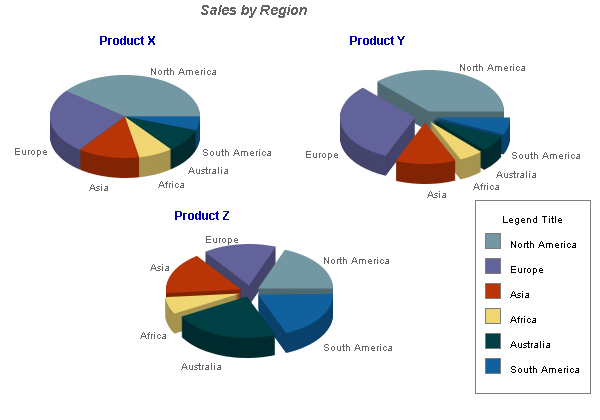
\includegraphics[width=.8\textwidth]{images/servlet3.png}
  \caption[A Pie chart]{Stolen from the net. Google for a pie chart...}
  \label{fig:pie}
\end{figure}

Many graphics packages can produce pdf files.
Embedded postscript (file extension .eps) are also a good candidate,
after converting them to pdf with the epstopdf tool. By the way: the
native format of Adobe Illustrator (ai) is similar enough to eps, so
that too can be processed with \texttt{ps2pdf}. Programs like {\em Visual
  Paradigm} can produce pdf files too. Sometimes open-office can
lend a helping hand. For instance, by cutting and pasting a Windows graphics into a single page OOdraw drawing, you can produce a very usable pdf file. 

Bitmap file types like png and jpeg take up a lot of space in your
final pdf document. 
Bitmap files take even more space if encoded into a pdf file.
As much as possible, stick to pdf (if necessary derived from svg or eps files). 

%\clearpage%to show headers

\section{A png example}
\label{page:pngexample}
If latex cannot fit the diagram on this page (page~\pageref{page:pngexample}), 
 then you may find the diagram as figure~\vref{fig:pie}. And as you
 can see, you can easily reference pages and images.

%\clearpage%to show headers
\section{PDF from a UML package} 
\label{sec:pdffromuml}
% Note how this varioref expands to
% something like on the next page.
% and using a wrapfigure
\begin{wrapfigure}{r}{.4\textwidth}
  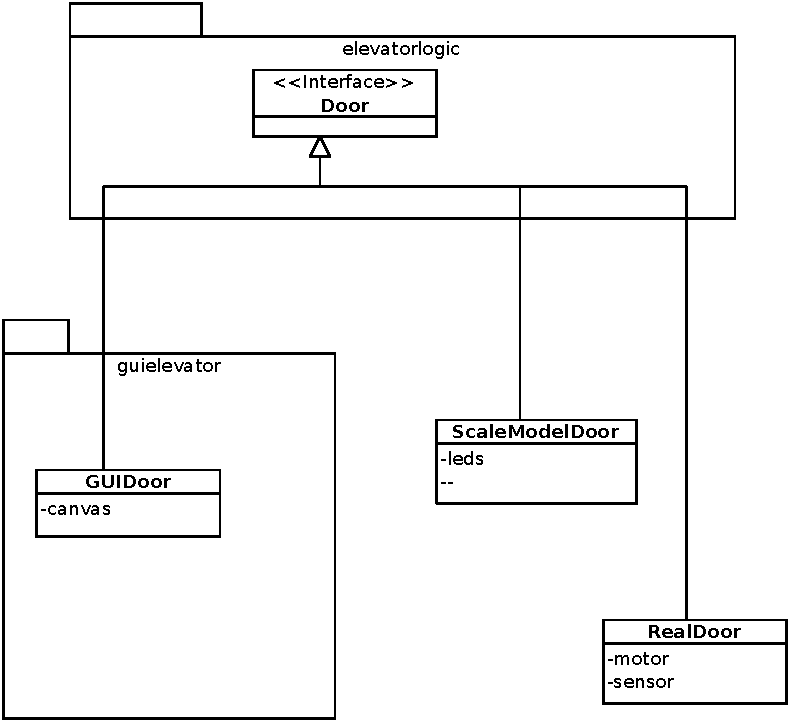
\includegraphics[width=.4\textwidth]{images/doorsystem.pdf}
  \caption{A class diagram made with Visual Paradigm}
  \label{fig:classdiagram}
\end{wrapfigure}
If the documentation you write is a design document of some software
package, you may want to include design diagrams.
No software engineering without a \define{\gls{UML}} diagrams\ldots.
You can see one generated with ``dia'', a vector drawing program that
understands the UML in figure~\ref{fig:classdiagram}
~\vpageref{fig:classdiagram}. This diagram is 'wrapped' in a \Code{wrapfigure} environment, so the text may flow around it

The diagram is not very sophisticated but shows an example of a vector
format file included via an eps$\rightarrow$ pdf conversion by
\texttt{epstopdf}.

Open source programs like Umlet, but also commercial ones like Visual Paradigm are also able to produce vector format graphics files. And sometimes it is helpful to add a box that is a bit bigger than the picture you want to include.
This ensures that the \define{\gls{boundingbox}} does not cut off any lines
you want in your picture. Sometimes it is necessary to give these
tools a helping hand with Inkscape, that is, do some tinkering to
get all the details right. Or with \Code{pdfcrop} which typically comes with your \LaTeX installation.

\begin{figure}[htbp]
  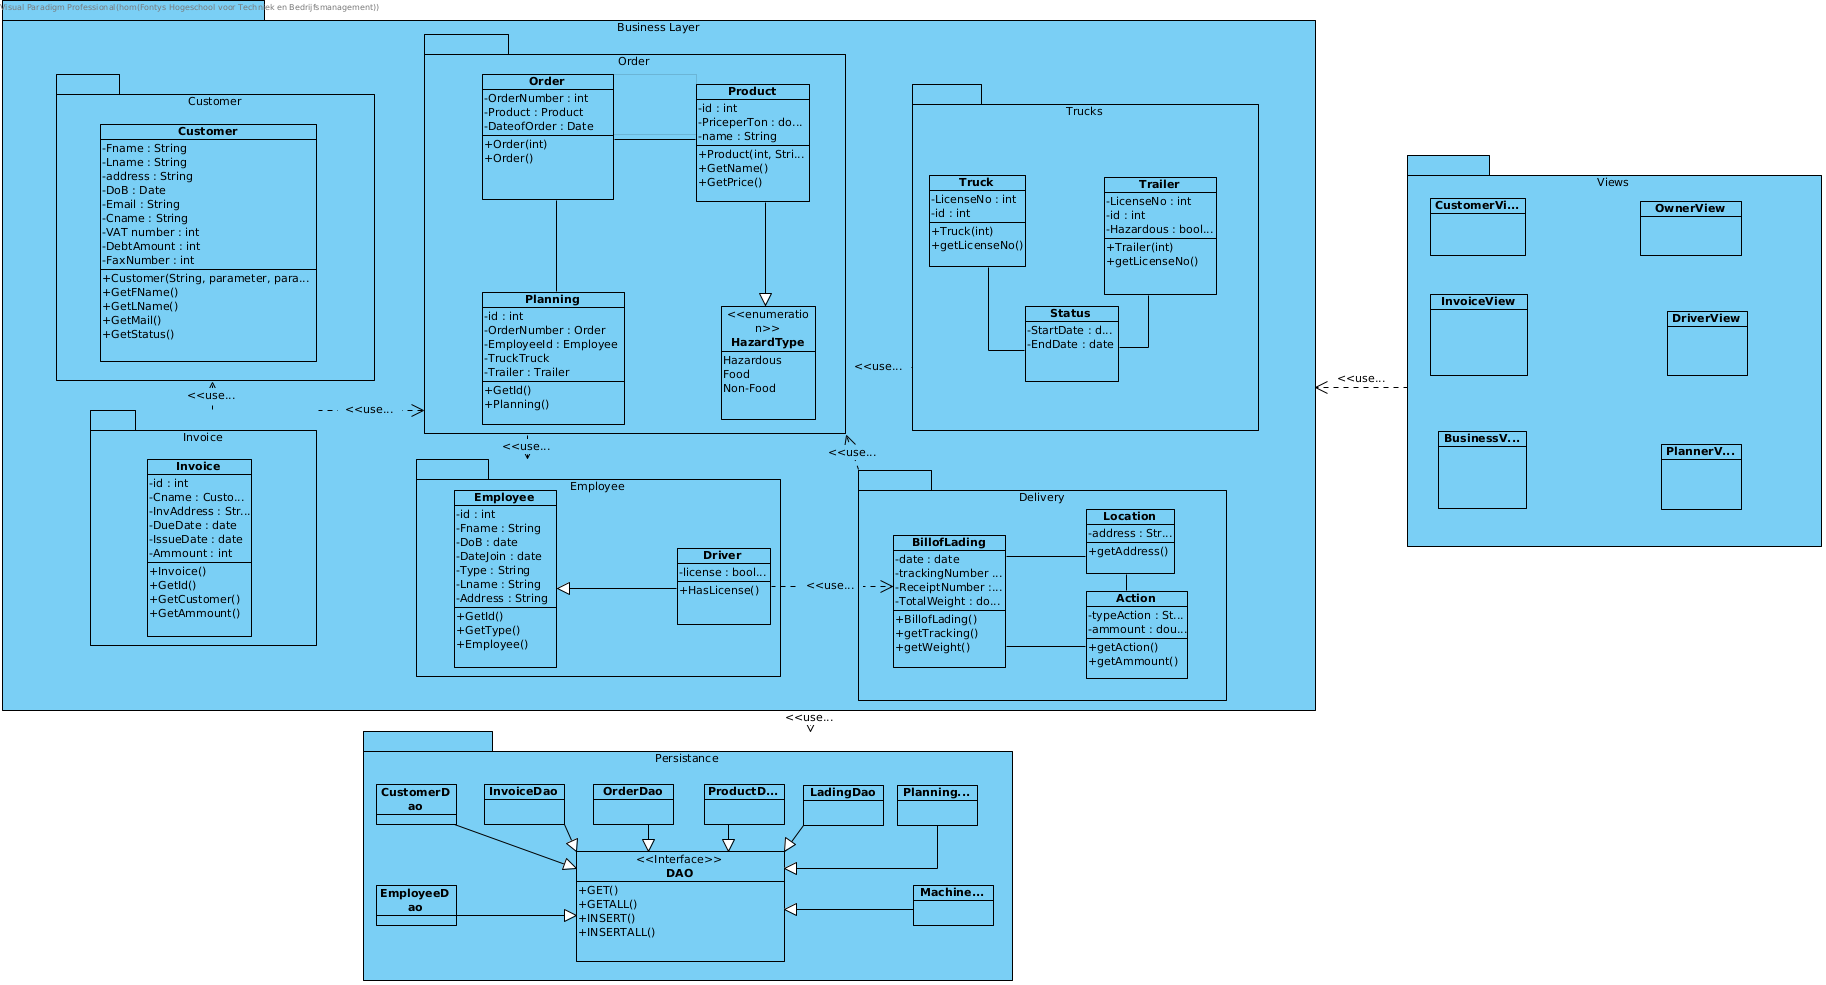
\includegraphics[width=\linewidth]{images/ClassDiagram1.png}
  \caption{You have been warned, NO PNG}
\end{figure}

The picture above is wrong on many fronts.
\begin{Itemize}
\item it uses PNG as the image format, whereas a vector format is provided by Visual Paradigm.
However, when you like a pixellated world such as in the game \gls{minecraft}, you will feel right at home if you zoom in a bit.
\item The arrows point in all directions, which is bad style. A proper UML class diagram should be stylish to improve comprehensibility, as it is recognizable at a glance. Think of Da Vinci's Vitruvian man.
\item It has the VPP blues, that is the colors used are completely non-functional, and also impair readability because the used color lowers the contract.
\end{Itemize}

Look on the next page how it is done properly.

% \begin{wrapfigure}{r}{.4\textwidth}
%   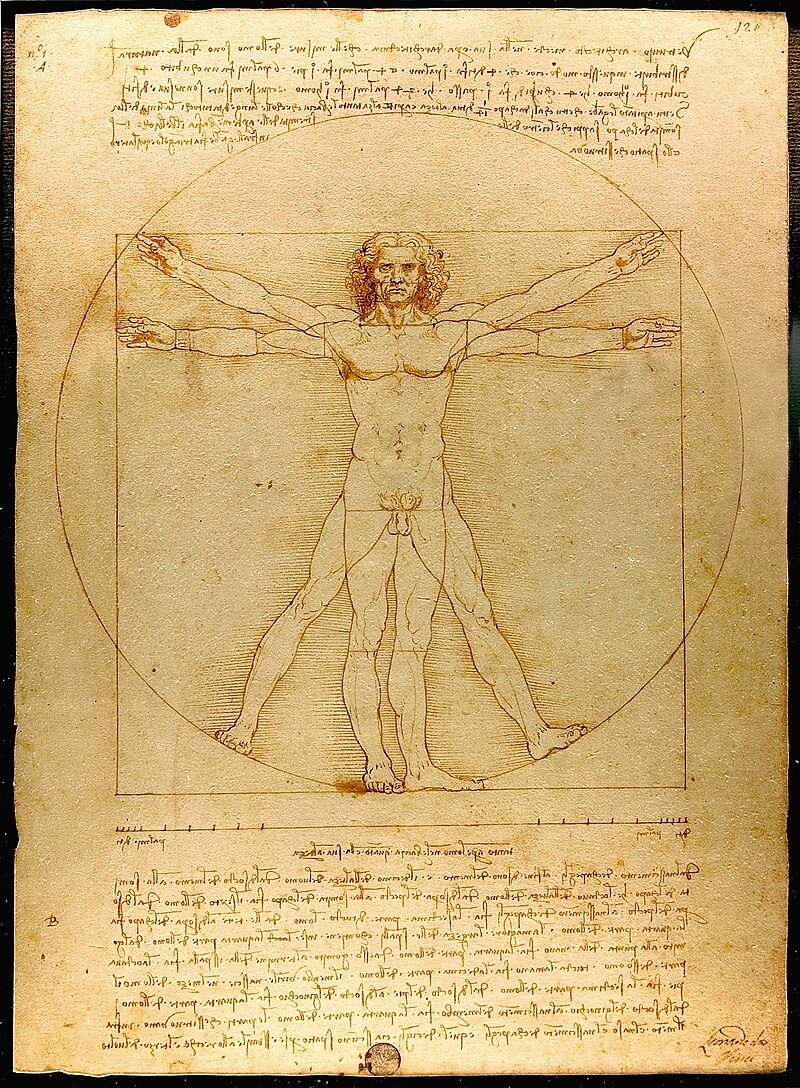
\includegraphics[width=.4\textwidth]{images/Da_Vinci_Vitruve_Luc_Viatour.jpg}
%   \caption{Left/right is has, up/down is inheritance (jpeg image)}
% \end{wrapfigure}
%\clearpage
\begin{figure}
  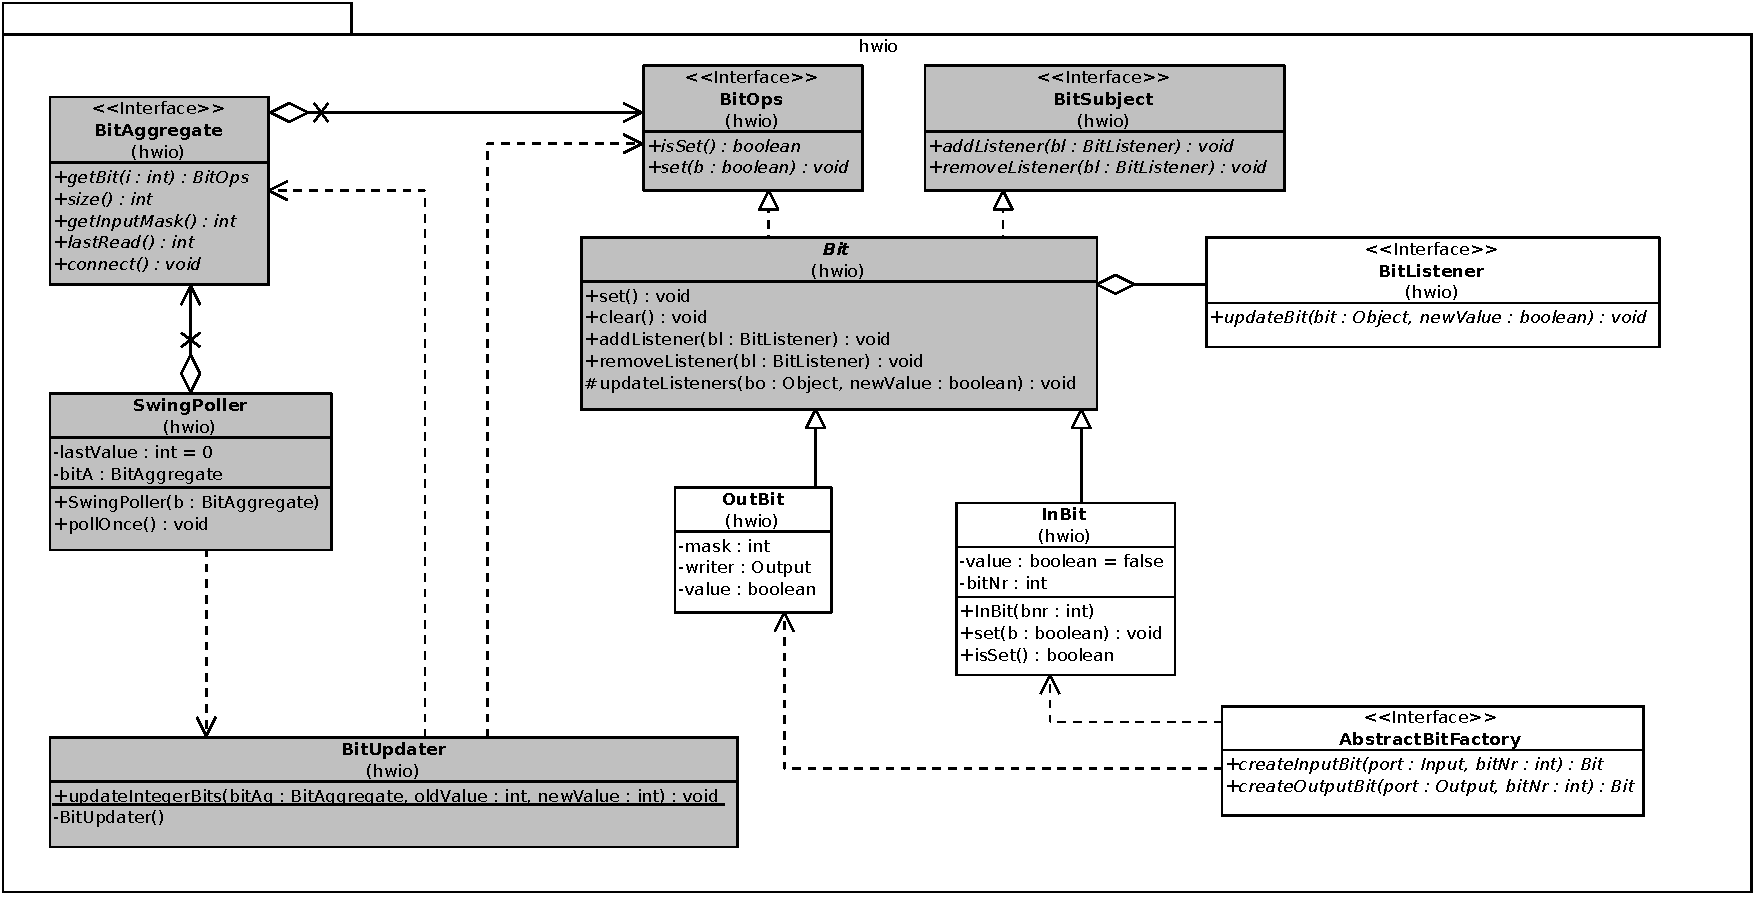
\includegraphics[width=\linewidth]{images/HWIO.pdf}
	\caption{UML made with Visual Paradigm, exported to SVG and then adapted with Inkscape and in the end exported to pdf}
\end{figure}

\begin{figure}[htbp]
  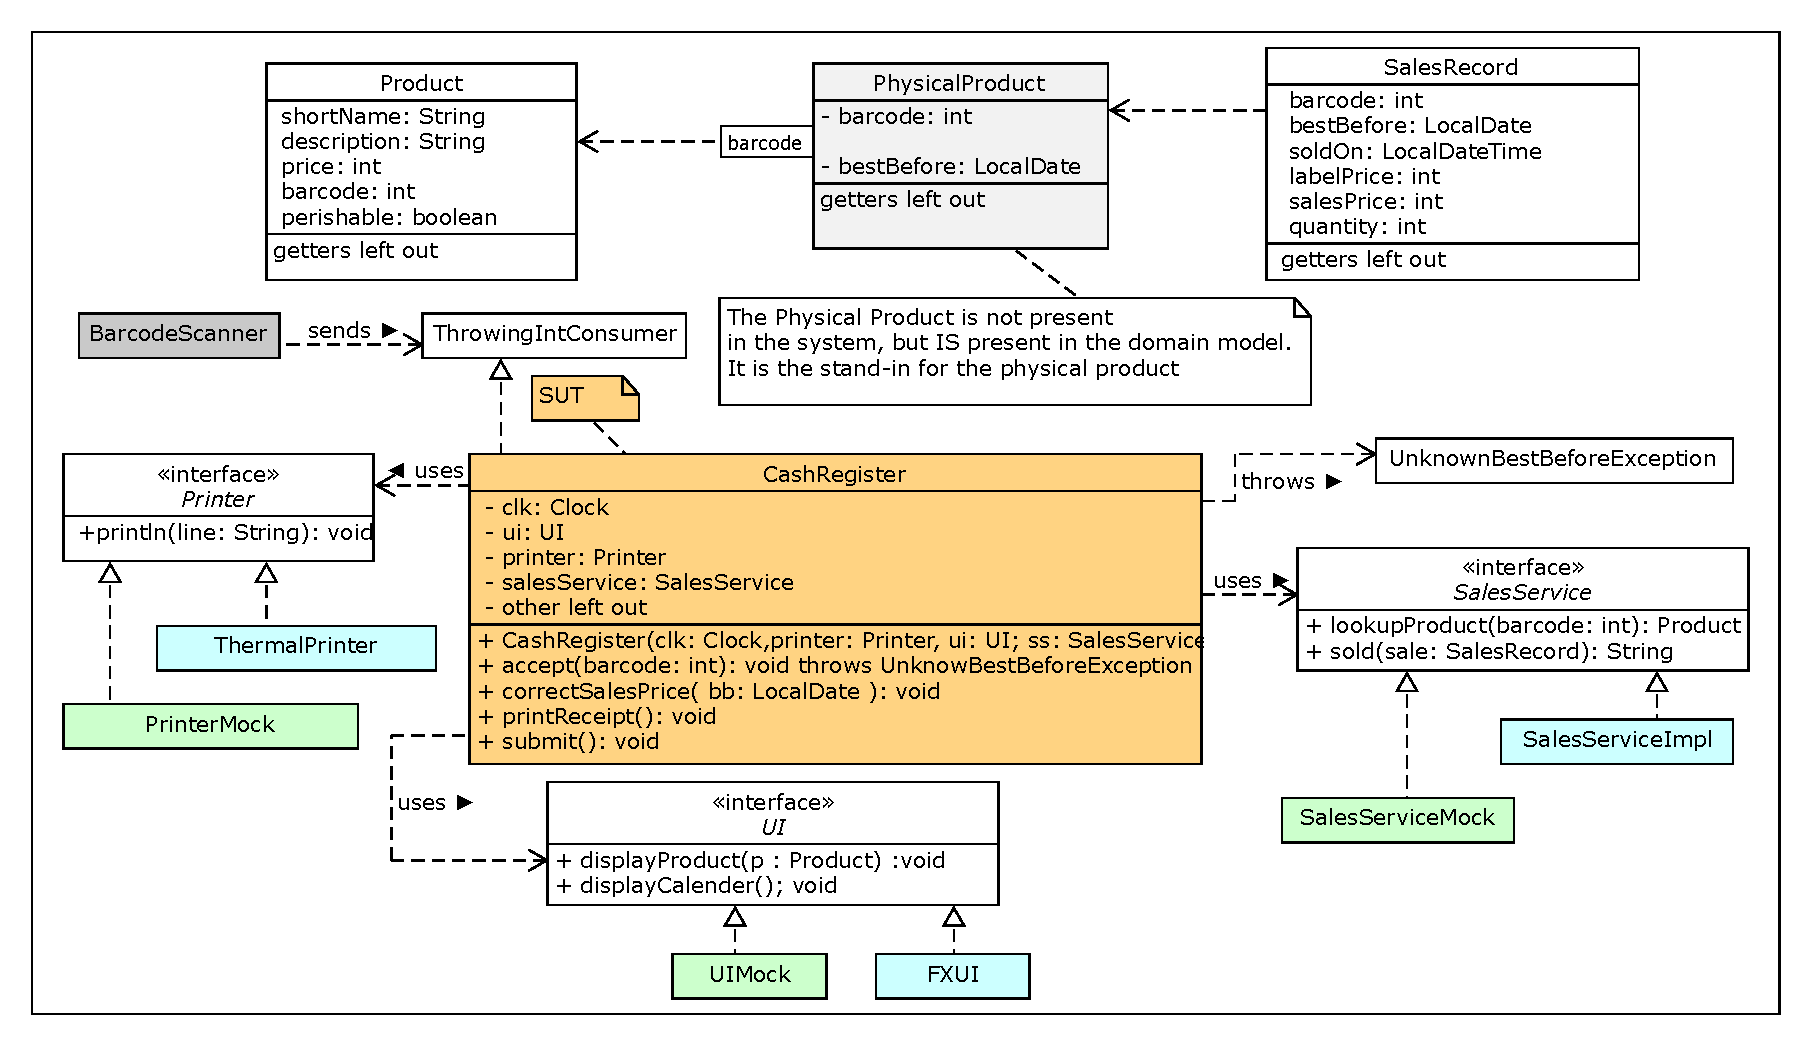
\includegraphics[width=\linewidth]{images/perishablesales.pdf}
  \caption{\label{fig:cashregistertest}Vector format (exported as pdf), with functional color and a legend, Made with Umlet}
\end{figure}


\subsection{Stylish UML Class diagram}
\label{sec:stylish}
Figure~\vref{fig:cashregistertest} above has style and uses functional colors which are easily explained with a legend.

Good style in a class diagram means:
\begin{Itemize}
\item There is always a direction. Arrows or triangles. They express dependencies.
\item Inheritance in the vertical direction only.
  \begin{Itemize}
    \item Any line that leaves at the top of a class box implies that this
      implements (dashed line) or extends (solid line), without looking where the line ends.
    \item Any triangle that enters at the bottom says that this class is extended or implemented for interfaces.
  \end{Itemize}
  \item All other relationships enter or leave at the left or right edge of the box, so you know things are used
  or this class is used/known.
  \begin{Itemize}
  \item If the local name is relevant, then that name is at the side of the using class, like the barcode at the PhysicalProduct which identifies a Product in the system. Internally the barcode is a simple number like an \Code{int} or a \Code{long}.
  \end{Itemize}
\end{Itemize}

Other than style there are other advantages to this kind of diagram.
\begin{Itemize}
\item You can zoom in as much as your viewer allows without getting a \define{\gls{minecraft}} world or worse.
\item A reviewer (the examiner, your coach or someone working with your documents) can select the texts in the diagram and can mark it. You too could do that to embellish the diagram.
\item There is no way you can do that nicely with a pixel based format like PNG or JPEG.
\end{Itemize}

This last diagram has been made with UMLet.

%%% Local Variables: 
%%% mode: latex
%%% TeX-master: "main"
%%% End: 
